\chapter{Introduction}
\label{ch:introduction}

\section{Background and Motivation}
Modern payment platforms process millions of transactions daily, each subject to complex validation rules that protect customers, reduce operational risk, and ensure regulatory compliance. At Deutsche Bank's eBridge-EU system, these Kotlin code validation rules span from simple field validations (mandatory characters, allowed value sets) to intricate domain-specific constraints (country-specific limits, routing conditions, SWIFT/ISO message-format requirements). With hundreds of rules evolving continuously across distributed teams and systems, developers and quality assurance teams face a critical challenge: quickly finding and understanding the exact rules relevant to their current task.

Traditional keyword search fails this use case. Rules are described inconsistently across teams, terminology overlaps, and natural language queries rarely match the exact vocabulary in rule documentation. A developer asking about ``EUR cross-border limits'' might miss rules titled ``SEPA maximum amount validation'' despite their relevance. Moreover, rule data is often scattered across multiple systems, with inconsistent formats and outdated versions. Simultaneously, banking environments impose strict architectural constraints: no external API calls, limited infrastructure dependencies, and complete audit trails for all data access.

This thesis presents a full-stack Retrieval-Augmented Generation (RAG) system that addresses these challenges through a pragmatic, monolithic architecture. Built as a single Dash application, the system combines modern NLP techniques with banking-compliant infrastructure constraints. We implement RAG's retrieval component using a hybrid approach—blending lexical (BM25), fuzzy string matching, and semantic (dense embeddings) signals—while the generation component provides grounded explanations drawn directly from stored fields, avoiding any query-time LLM calls.

The key innovation lies in the system's \emph{CSV-first} design coupled with comprehensive data standardization. We consolidated scattered rule data from multiple distributed sources into a single, clean CSV corpus with standardized fields and consistent formatting. This CSV serves as both the source of truth and the operational datastore, with all rule data—including 1024-dimensional embeddings stored as JSON strings—in one authoritative file. At startup, the system ingests this CSV into an SQLite database for efficient querying and builds in-memory indices for each retrieval signal. This architecture eliminates complex dependencies (no FAISS, no external vector databases) while maintaining sub-second query latency through careful indexing with \texttt{scikit-learn} and \texttt{rank\_bm25}. The monolithic Dash architecture ensures the entire application—from data ingestion through retrieval, ranking, and UI rendering—runs as a single Python process, simplifying deployment and audit compliance in regulated environments.

\section{Problem Statement}
\textbf{Goal.} Given a user query about a Kotlin code validation rule (e.g., ``EUR cross-border limit'' or ``party agent checks for DE''), the system should:
\begin{enumerate}[leftmargin=*,itemsep=2pt,topsep=2pt]
 \item return a short, ranked list of relevant rules drawn from a \emph{single, standardized CSV corpus};
 \item display all available rule information (codes, tags, language variants, Kotlin code) and a short, factual explanation grounded in the stored fields;
 \item respect banking constraints (no external vector DBs, no FAISS) and meet a sub-second target for typical searches.
\end{enumerate}

\section{Corpus and Fields}
Each row in the standardized CSV represents one Kotlin validation rule, consolidated from distributed sources and cleaned to ensure consistency:
\begin{itemize}[leftmargin=*,itemsep=2pt,topsep=2pt]
 \item \textbf{Identifiers}: \textit{Rule ID, Rule Name} (deduplicated across sources).
 \item \textbf{Business descriptions}: \textit{English Description, German Description} (standardized terminology).
 \item \textbf{Error codes}: \textit{BANSTA Error Code, ISO Error Code} (validated against official registries).
 \item \textbf{LLM-enriched text}: \textit{LLM Generated Description} (created offline for clarity and completeness).
 \item \textbf{Search fields}: \textit{Keywords} (curated terms), \textit{Tags} (Rule Type, Country, Business Type, Party Agent).
 \item \textbf{Metadata}: \textit{Relevance} (a rule-level score in $[0,1]$), \textit{Embedding} (JSON string with 1024 floats), \textit{Versioning}, \textit{Date}.
 \item \textbf{Implementation}: \textit{Kotlin Code} (the actual validation rule implementation).
\end{itemize}
Embeddings are produced with \texttt{UAE-Large-V1} (1024 dimensions, mean pooling), L2-normalized, and stored as JSON strings. The bilingual fields (EN/DE) support business users across teams while keeping a single source of truth. This standardization process resolved inconsistencies in naming conventions, merged duplicate rules, and established canonical representations for all fields.

\section{System Overview}
The monolithic Dash application implements a complete RAG pipeline with intentionally minimal dependencies and efficient startup initialization:

\begin{itemize}[leftmargin=*,itemsep=2pt,topsep=2pt]
 \item \textbf{Data Layer}: CSV ingestion into SQLite at startup, JSON embedding parsing into numpy arrays, L2 normalization, in-memory caching of all indices.
 \item \textbf{Retrieval Layer}: Three parallel retrievers initialized at startup—BM25 index (via \texttt{rank\_bm25}) over keywords, fuzzy matcher (via \texttt{fuzzywuzzy}) on rule names, and semantic search (via \texttt{scikit-learn}'s \texttt{cosine\_similarity}) on the embedding matrix. 
 \item \textbf{Ranking Layer}: Per-query score normalization, convex combination with tuned weights, semantic gating at $\tau=0.30$.
 \item \textbf{UI Layer}: Dash components for mode selection (Keyword/Hybrid), faceted filtering, ranked result cards displaying all available rule information including Kotlin code with tag badges, and grounded explanation panels rendered from stored fields.
 \item \textbf{No External Dependencies}: No FAISS, no vector databases, no query-time LLM calls, no network requests during search—all computation happens in-process.
\end{itemize}

\begin{figure}[t]
\centering
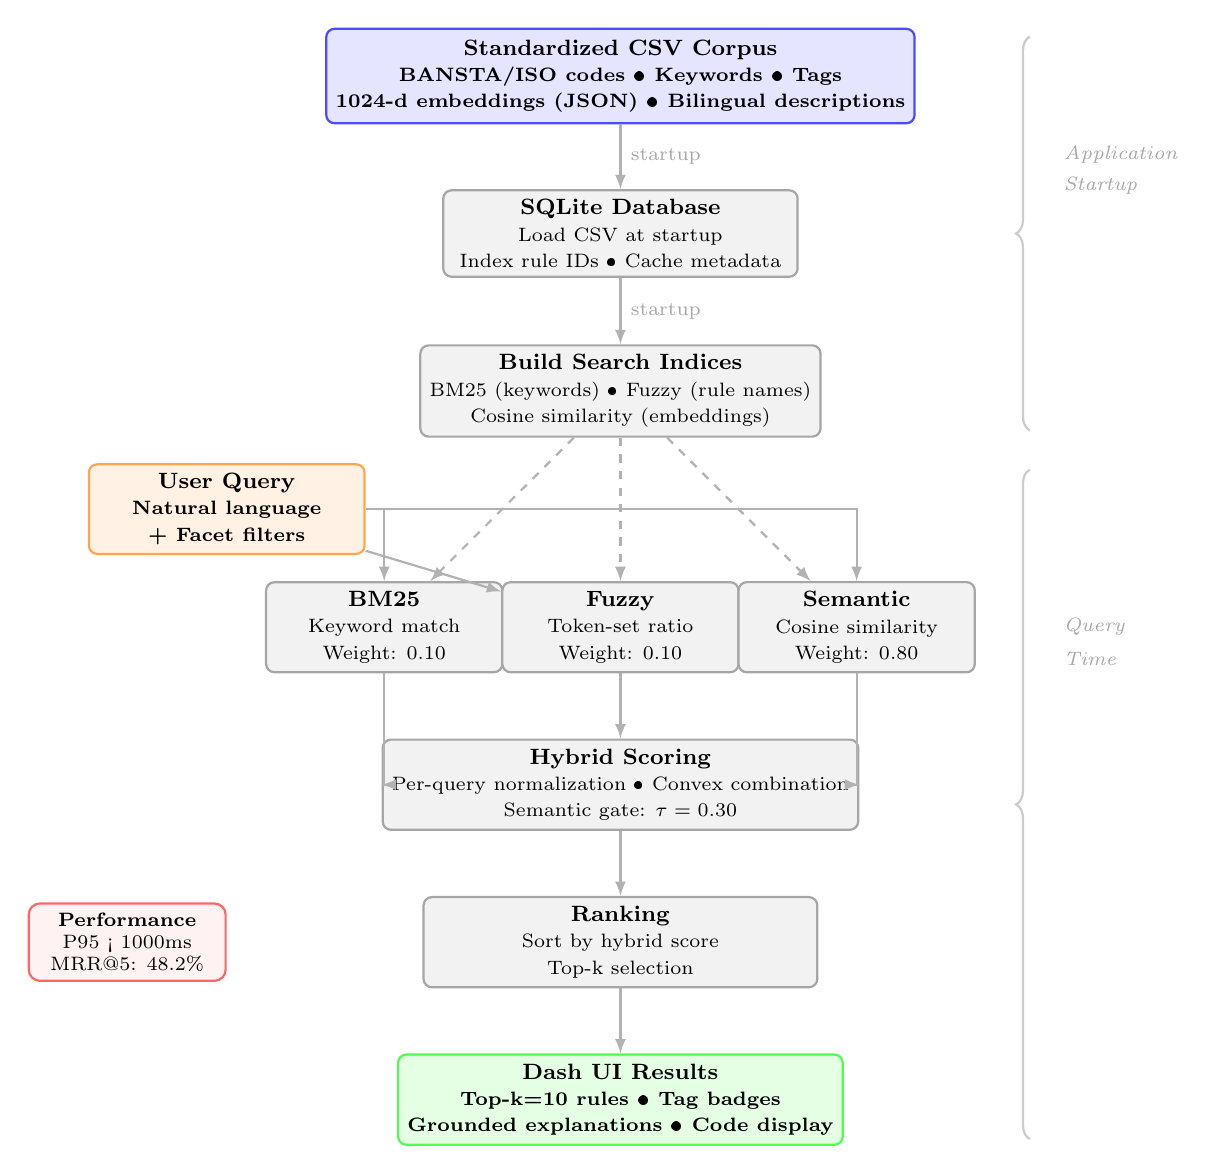
\begin{tikzpicture}[
 >=latex,
 thick,
 font=\footnotesize,
 % Node styles
 datanode/.style={
   draw=blue!70, 
   fill=blue!10, 
   rounded corners=3pt, 
   minimum width=5cm, 
   minimum height=1.2cm, 
   align=center,
   font=\footnotesize\bfseries
 },
 processnode/.style={
   draw=gray!70, 
   fill=gray!10, 
   rounded corners=3pt, 
   minimum width=4.5cm, 
   minimum height=1cm, 
   align=center,
   font=\footnotesize
 },
 querynode/.style={
   draw=orange!70, 
   fill=orange!10, 
   rounded corners=3pt, 
   minimum width=3.5cm, 
   minimum height=0.9cm, 
   align=center,
   font=\footnotesize\bfseries
 },
 resultnode/.style={
   draw=green!70, 
   fill=green!10, 
   rounded corners=3pt, 
   minimum width=4.5cm, 
   minimum height=1cm, 
   align=center,
   font=\footnotesize\bfseries
 },
 arrow/.style={->, thick, draw=gray!60},
 dashedarrow/.style={->, thick, draw=gray!60, dashed},
 label/.style={font=\scriptsize, text=gray!70}
]

% Main vertical flow
\node[datanode] (csv) at (0,0) {
 \textbf{Standardized CSV Corpus}\\
 \scriptsize BANSTA/ISO codes • Keywords • Tags\\
 \scriptsize 1024-d embeddings (JSON) • Bilingual descriptions
};

\node[processnode] (sqlite) at (0,-2) {
 \textbf{SQLite Database}\\
 \scriptsize Load CSV at startup\\
 \scriptsize Index rule IDs • Cache metadata
};

\node[processnode] (indices) at (0,-4) {
 \textbf{Build Search Indices}\\
 \scriptsize BM25 (keywords) • Fuzzy (rule names)\\
 \scriptsize Cosine similarity (embeddings)
};

% User query enters from left
\node[querynode] (query) at (-5,-5.5) {
 \textbf{User Query}\\
 \scriptsize Natural language\\
 \scriptsize + Facet filters
};

% Three parallel retrieval paths
\node[processnode, minimum width=3cm] (bm25) at (-3,-7) {
 \textbf{BM25}\\
 \scriptsize Keyword match\\
 \scriptsize Weight: 0.10
};

\node[processnode, minimum width=3cm] (fuzzy) at (0,-7) {
 \textbf{Fuzzy}\\
 \scriptsize Token-set ratio\\
 \scriptsize Weight: 0.10
};

\node[processnode, minimum width=3cm] (semantic) at (3,-7) {
 \textbf{Semantic}\\
 \scriptsize Cosine similarity\\
 \scriptsize Weight: 0.80
};

% Scoring and ranking
\node[processnode, minimum width=5cm] (hybrid) at (0,-9) {
 \textbf{Hybrid Scoring}\\
 \scriptsize Per-query normalization • Convex combination\\
 \scriptsize Semantic gate: $\tau = 0.30$
};

\node[processnode, minimum width=5cm] (rank) at (0,-11) {
 \textbf{Ranking}\\
 \scriptsize Sort by hybrid score\\
 \scriptsize Top-k selection
};

\node[resultnode] (results) at (0,-13) {
 \textbf{Dash UI Results}\\
 \scriptsize Top-k=10 rules • Tag badges\\
 \scriptsize Grounded explanations • Code display
};

% Arrows for main flow
\draw[arrow] (csv) -- node[right, label] {startup} (sqlite);
\draw[arrow] (sqlite) -- node[right, label] {startup} (indices);

% Query flows
\draw[arrow] (query) -| (bm25);
\draw[arrow] (query) -- (fuzzy);
\draw[arrow] (query) -| (semantic);

% Indices connection (dashed to show pre-built)
\draw[dashedarrow] (indices) -- (bm25);
\draw[dashedarrow] (indices) -- (fuzzy);
\draw[dashedarrow] (indices) -- (semantic);

% Convergence to hybrid
\draw[arrow] (bm25) |- (hybrid);
\draw[arrow] (fuzzy) -- (hybrid);
\draw[arrow] (semantic) |- (hybrid);

% Final flow
\draw[arrow] (hybrid) -- (rank);
\draw[arrow] (rank) -- (results);

% Add timing annotations
\node[label, anchor=west] at (5.5,-1) {\textit{Application}};
\node[label, anchor=west] at (5.5,-1.4) {\textit{Startup}};
\draw[gray!40, thick, decorate, decoration={brace, amplitude=5pt, mirror}] 
 (5.2,0.5) -- (5.2,-4.5);

\node[label, anchor=west] at (5.5,-7) {\textit{Query}};
\node[label, anchor=west] at (5.5,-7.4) {\textit{Time}};
\draw[gray!40, thick, decorate, decoration={brace, amplitude=5pt, mirror}] 
 (5.2,-5) -- (5.2,-13.5);

% Add performance annotation
\node[draw=red!60, fill=red!5, rounded corners, anchor=east, 
     font=\scriptsize, align=center, minimum width=2.5cm] 
     at (-5,-11) {
 \textbf{Performance}\\
 P95 < 1000ms\\
 MRR@5: 48.2\%
};

\end{tikzpicture}
\caption{Monolithic RAG architecture with vertical data flow. The system follows a clear pipeline from data ingestion at startup through query-time retrieval and ranking. The three retrieval signals (BM25, Fuzzy, Semantic) operate in parallel with empirically tuned weights from LOOCV evaluation. All components run in-process within a single Dash application, with no external dependencies.}
\label{fig:intro-architecture}
\end{figure}

\section{Retrieval Modes and Scoring}
\paragraph{Keyword mode (BM25).} We index the \emph{Keywords} field at startup and compute BM25 scores for queries. This mode is deterministic and fast, performing well when query vocabulary matches the curated keywords.

\paragraph{Hybrid mode (three signals).} For each candidate rule $r$ with keywords $K(r)$ and LLM description $D(r)$:
\[
s_{\text{kw}} = \mathrm{BM25}(q, K(r)),\quad
s_{\text{fuzzy}} = \tfrac{1}{100}\,\mathrm{TokenSetRatio}(q, \mathrm{name}(r)),\quad
s_{\text{sem}} = \cos\!\big(\phi(q), \psi(D(r))\big),
\]
where $\phi$ and $\psi$ are \texttt{UAE-Large-V1} encoders (1024-d, mean pooling). Scores are min–max normalized per query across the candidate pool to $[0,1]$. We apply a semantic gate to filter obviously off-topic results:
\[
s_{\text{sem}}' = \begin{cases}
s_{\text{sem}} & \text{if } s_{\text{sem}} \ge \tau \\
0 & \text{otherwise}
\end{cases}
\quad \text{with} \quad \tau = 0.30.
\]
The final score is a convex combination with weights empirically tuned via Leave-One-Out Cross-Validation (LOOCV):
\[
\boxed{ \; s \;=\; 0.10\,\widehat{s}_{\text{kw}} \;+\; 0.10\,\widehat{s}_{\text{fuzzy}} \;+\; 0.80\,\widehat{s}_{\text{sem}}' \; }.
\]
These weights maximize Mean Reciprocal Rank at 5 (MRR@5) on our evaluation dataset, improving from 43.4\% (initial weights) to 48.2\% (tuned weights).

\paragraph{Why this design works.} The hybrid approach balances precision and coverage:
\begin{itemize}[leftmargin=*,itemsep=2pt,topsep=2pt]
 \item BM25 anchors results in the curated vocabulary from the standardized corpus.
 \item Fuzzy matching tolerates minor spelling or tokenization differences in rule names.
 \item Semantic similarity captures meaning when wording diverges but intent remains aligned.
 \item The semantic gate ($\tau=0.30$) reduces noise from accidental token overlaps.
 \item SQLite provides efficient filtering and sorting without external database dependencies.
 \item Pre-built indices at startup eliminate query-time index construction overhead.
\end{itemize}

\section{Operational Constraints and Non-Goals}
\paragraph{Constraints.} The system is designed for a regulated banking environment:
\begin{itemize}[leftmargin=*,itemsep=2pt,topsep=2pt]
 \item \textbf{No FAISS or external vector stores}. Dense similarity uses \texttt{scikit-learn}'s \texttt{cosine\_similarity} on the embedding matrix (i.e., normalized dot product) with in-memory vectors parsed from the CSV's JSON embedding field at startup.
 \item \textbf{No query-time LLM expansion}. All LLM processing (generating descriptions, extracting keywords) happens offline during corpus standardization. Query-time explanations are assembled from pre-stored fields only.
 \item \textbf{Latency requirement}. P95 latency must remain under 1000ms for top-$k{=}10$ retrieval on the full corpus (${\sim}10^3$ rules), measured end-to-end from query submission to UI render.
 \item \textbf{Single-file deployment}. The entire rule corpus, including embeddings, must remain in a single CSV file for audit and version control purposes.
\end{itemize}
\paragraph{Non-goals.} The system does not execute validation rules, analyze Kotlin source code, or validate runtime behavior. Its sole purpose is \emph{information retrieval} and \emph{grounded explanation} over the standardized tabular rule corpus.

\section{Research Questions}
\begin{description}[leftmargin=!,labelwidth=2.5cm,itemsep=2pt,topsep=2pt]
 \item[RQ1:] What is the optimal weight configuration for hybrid retrieval, and how much does it improve MRR@5 over individual signals?
 \item[RQ2:] How robust is performance to weight perturbations, and what is the contribution of each signal in ablation studies?
 \item[RQ3:] Does the semantic gate ($\tau{=}0.30$) effectively filter noise while preserving relevant results?
 \item[RQ4:] Can the system maintain P95 latency under 1000ms while serving concurrent users in a production Dash deployment?
\end{description}

\section{Contributions}
\begin{enumerate}[leftmargin=*,itemsep=2pt,topsep=2pt]
 \item A production-ready, monolithic RAG system for Kotlin code validation rule retrieval that operates within strict banking infrastructure constraints—no FAISS, no external vector databases, no query-time LLM calls.
 \item A comprehensive data standardization pipeline that consolidated distributed, inconsistent rule sources into a single, clean CSV corpus with uniform field definitions and validated error codes.
 \item An empirically optimized hybrid retrieval approach with LOOCV-tuned weights (semantic 0.80, BM25 0.10, fuzzy 0.10) and semantic gating ($\tau{=}0.30$).
 \item A complete full-stack implementation in Dash with efficient startup initialization—SQLite ingestion and index building—demonstrating that sophisticated NLP capabilities can be delivered through simple, auditable architectures.
 \item Rigorous evaluation using Leave-One-Out Cross-Validation showing 48.2\% MRR@5, with detailed ablation studies and sensitivity analyses confirming robustness.
 \item A CSV-first data architecture that stores 1024-dimensional embeddings as JSON strings, enabling single-file deployment while maintaining sub-second query performance through in-memory indexing.
\end{enumerate}

\section{Thesis Structure}
The remainder of this thesis is organized as follows. \textbf{Chapter~2 (Fundamentals)} introduces the theoretical background of information retrieval, covering BM25 scoring, fuzzy string matching, dense embeddings with UAE-Large-V1, and the Retrieval-Augmented Generation (RAG) pattern. \textbf{Chapter~3 (Related Work)} situates the project within prior research on hybrid retrieval and rule discovery in financial contexts, highlighting gaps that motivate the present system. \textbf{Chapter~4 (Corpus Analysis)} examines the standardized rule corpus, including field completeness, tag distributions, and embedding quality after consolidation. \textbf{Chapter~5 (System Design)} presents the architecture of the retrieval system, detailing the hybrid scoring function, per-query normalization, SQLite integration, and the monolithic Dash application. \textbf{Chapter~6 (Implementation)} describes the Python codebase, initialization sequence, and key design choices that enable efficient in-memory operation without external dependencies. \textbf{Chapter~7 (Evaluation)} reports experimental results using LOOCV, ablation studies, and sensitivity analyses to assess retrieval performance. Finally, \textbf{Chapter~8 (Conclusion)} summarizes the contributions, discusses limitations of the CSV-first approach, and outlines future directions such as graded relevance, neural re-ranking, and a chatbot interface.